\documentclass[12pt]{scrartcl}
\usepackage{float,  fullpage,url,verbatim,mathtools,amsmath,amssymb,latexsym,amsfonts,amsthm,hyperref}\setlength{\parskip}{3mm}\setlength{\parindent}{0mm}
\usepackage{color}
%\usepackage[demo]{graphicx}
%\usepackage{caption}
%\usepackage{subcaption}
\usepackage{graphicx}
\usepackage{subfig}
\usepackage{natbib}
\bibliographystyle{abbrvnat}
\setcitestyle{authoryear,open={(},close={)}}


\renewcommand{\baselinestretch}{1.2}

\pdfminorversion=4

% NOTATIONS
%%%%%%%%%%%%%
%%%%%%%%%%%%%
% Ensembles
\def\nset{{\mathbb{N}}}
\def\rset{\mathbb R}
\def\zset{\mathbb Z}
\def\qset{\mathbb Q}
\def\eqsp{\;}

\newcommand{\ie}{{\em i.e.} }
\newcommand{\as}{\text{a.s.} }
 \newcommand{\seq}[1]{\left<#1\right>}
 \newcommand{\pscal}[2]{\left\langle#1,#2\right\rangle}

\newcommand{\un}{\ensuremath{\mathbbm{1}}}
\newcommand{\eqdef}{\ensuremath{\stackrel{\mathrm{def}}{=}}}
\newcommand{\eps}{\varepsilon}


\def\Xset{\mathsf{X}} % Espace d 'etat
\def\Vset{\mathsf{V}} % Espace d 'etat
\def\Yset{\mathsf{Y}} % Espace d 'etat
\def\Xsigma{\mathcal{X}} % tribu sur X
\def\Tsigma{\mathcal{B}(\Theta)} % tribu sut Theta
\def\F{\mathcal{F}} % filtration
\def\B{\mathcal{B}} % filtration
\def\barB{\overline{B}} % filtration
\def\Lip{\textsf{Lip}}
\def\e{\mathcal{E}}
\def\dist{\textsf{d}}
\def\E{\mathbb{E}}
\def\S{\mathcal{S}}
\def\N{\mathcal{N}}
\def\M{\mathcal{M}}
\def\Mt{\mathcal{M}_{2,\textsf{w}}^{(0)}}
\def\G{\mathbb{G}}
\def\A{\mathcal{A}}
\def\H{\mathcal{H}}
\def\cov{\mathbb{C}\mbox{ov}}





\def\PP{\mathbb{P}} % proba
\def\PE{\mathbb{E}} % esperance
\def\bPP{\overline{\mathbb{P}}} % proba sur espace double
\def\bPE{\overline{\mathbb{E}}} % esperance sur espace double
\def\cPP{\check{\mathbb{P}}} % proba sur espace quadruple
\def\cPE{\check{\mathbb{E}}} % esperance sur espace quadruple
\def\cP{\check{P}} % proba



\def\lyap{\omega}
\def\W{\mathcal{W}}
\def\K{\mathcal{K}}
\def\L{\mathcal{L}} % espace des fonctions
\def\Vs{V_\star}
\def\lip{\mathrm{Lip}}
\def\V{\mathbb{V}}
\def\ns{n_\star}
\def\tv{\mathrm{tv}}
\def\tauout{\stackrel{\leftarrow}{\tau}} % temps de sortie
\def\compact{\mathsf{K}}  % compact
\def\Cset{\mathcal{C}} % Petite set
\def\Dset{\mathcal{D}} % Generic set
\newcommand{\dlim}{\ensuremath{\stackrel{\mathcal{D}}{\longrightarrow}}}
\newcommand{\plim}[1]{\ensuremath{\stackrel{\mathrm{P}_{#1}}{\longrightarrow}}}
\newcommand{\aslim}{\ensuremath{\stackrel{\text{a.s.}}{\longrightarrow}}}
\newcommand\Plim[1]{\mathbb{Q}_{#1}}
\newcommand{\abs}[1]{\left\vert#1\right\vert}
\newcommand{\norm}[1]{\left\Vert#1\right\Vert}
\newcommand{\nnorm}[1]{\left\vert\!\left\vert\!\left\vert#1\right\vert\!\right\vert\!\right\vert}
\newcommand{\normfro}[1]{\left\Vert#1\right\Vert_{\textsf{F}}}
\newcommand{\inte}[1]{\stackrel{\circ}{#1}}
\def\Prox{\operatorname{Prox}}
\def\Proj{\operatorname{Proj}}
\newcommand{\ac}[1]{\textbf{#1}}

\def\Rg{\mathsf{Rg}}
\def\barlambda{\underline{\Lambda}}
\def\Mb{\mathcal{M}_\textsf{b}}
\def\b{\textsf{b}}
\def\I{\textsf{I}}
\def\t{\textsf{T}}
\def\w{\textsf{w}}
\def\c{\textsf{c}}
\def\deg{\textsf{deg}}

\usepackage{bm}%bold matH
\def\bzero{{\bf 0}}







% DIALOGUES ENTRE AUTEURS
%%%%%%%%%%%%%%%%%%%%%%%%%
%\newcommand{\comment}[2]{\begin{quote}\color{#1}\begin{sffamily} #2 \end{sffamily}\color{black}\end{quote}}
%\newcommand{\note}[2]{\marginpar{\parbox[t]{\noteWidth}{\raggedright\textcolor{blue}{\tiny{#2}} \textcolor{red}{\tiny{#1}}}}}

%\def\yves{blue}
%\newlength{\noteWidth}
%\setlength{\noteWidth}{.6in}


\providecommand{\keywords}[1]{\textbf{\textit{Keywords:}} #1}

%% THEO, HYP, LEM, PROP ...
%%%%%%%%%%%%%%%%%%%%%%%%%%%%%
\newenvironment{hyp}{\begin{itemize}
  \item[]}{\end{itemize}}
\newtheorem{theo}{Theorem}[section]
\newtheorem{lemma}[theo]{Lemma}
\newtheorem{coro}[theo]{Corollary}
\newtheorem{prop}[theo]{Proposition}
\newtheorem{defi}[theo]{Definition}
\newtheorem{algo}{Algorithm}[section]
\newtheorem{prob}{Open Problem}[section]
\newtheorem{hypo}{Assumption}[section]
%\theoremstyle{remark}
\newtheorem{rem}{Remark}
\newtheorem{example}{Example}


\title{Cloud Detection Literature Review}
%\date{}
\author{Chia Chye Yee, Yves Atchad\'e}
\begin{document}
\maketitle

\begin{abstract}
This is a literature review
\end{abstract}
\keywords{cloud detection, full convolutional neural networks, generative adversarial networks}


\section{Introduction} \label{sec:intro}

asdfdsf
%\section{Introduction to Convolutional Neural Networks} \label{sec:introductioncnn}

In this section, we will go over the basic concept of convolutional neural networks (CNN). For further reference, \cite{deshpande16} provides a very informative introduction. Simply, the problem statement is the task of assigning a class or a vector class probabilities given an image as an input. The image can be represented by a group of pixels. Each pixel can be represented as a vector of values for their red, green, blue (RGB) expressions which can range from 0 to 255. For instance, a red pixel can be represented by $(255, 0, 0)$, blue is $(0,0,255)$ etc. Based on this formulation of a digital image, we can represent an image by a data cube of values. As an example, an image with $32 \times 32$ pixels is a $32 \times 32 \times 3$ data cube.  This is taken as the input for the first convolutional layer.

\subsection{Convolutional Layers} \label{sec:convolayers}

For simplicity, suppose we consider only the red value from the array (ie. taking only the top layer of the aforementioned data cube -  a $32 \times 32$ matrix).
\section{Generative Adversarial Networks } \label{sec:gan}

The main reference for this paper is from \cite{zou2019}. We begin by motivating the methodology with a typical problem facing remote sensing images. Typically, images captured from satellites orbiting earth are attenuated by cloud covering making the information retrieval used in various applications challenging. Therefore, the research on cloud detection and its subsequent removal from images has received significant amount of attention in recent years \textcolor{red}{(add citation and further elaboration?)}. 

Although most of the research frame this problem as a pixel-level classification problem \textcolor{red}{(add citation)}, pixel-wise classification leads to category ambiguity for detection of semi-transparent clouds. In other words, the cloud probability output from convolutional networks for each pixel are often inconclusive for areas of the image covered by semi-transparent clouds. Recognizing this issue, the authors of cite{zou2019} recast the problem as mixed energy separation problem commonly referred to as image matting. 

\begin{figure}[h]
\centering
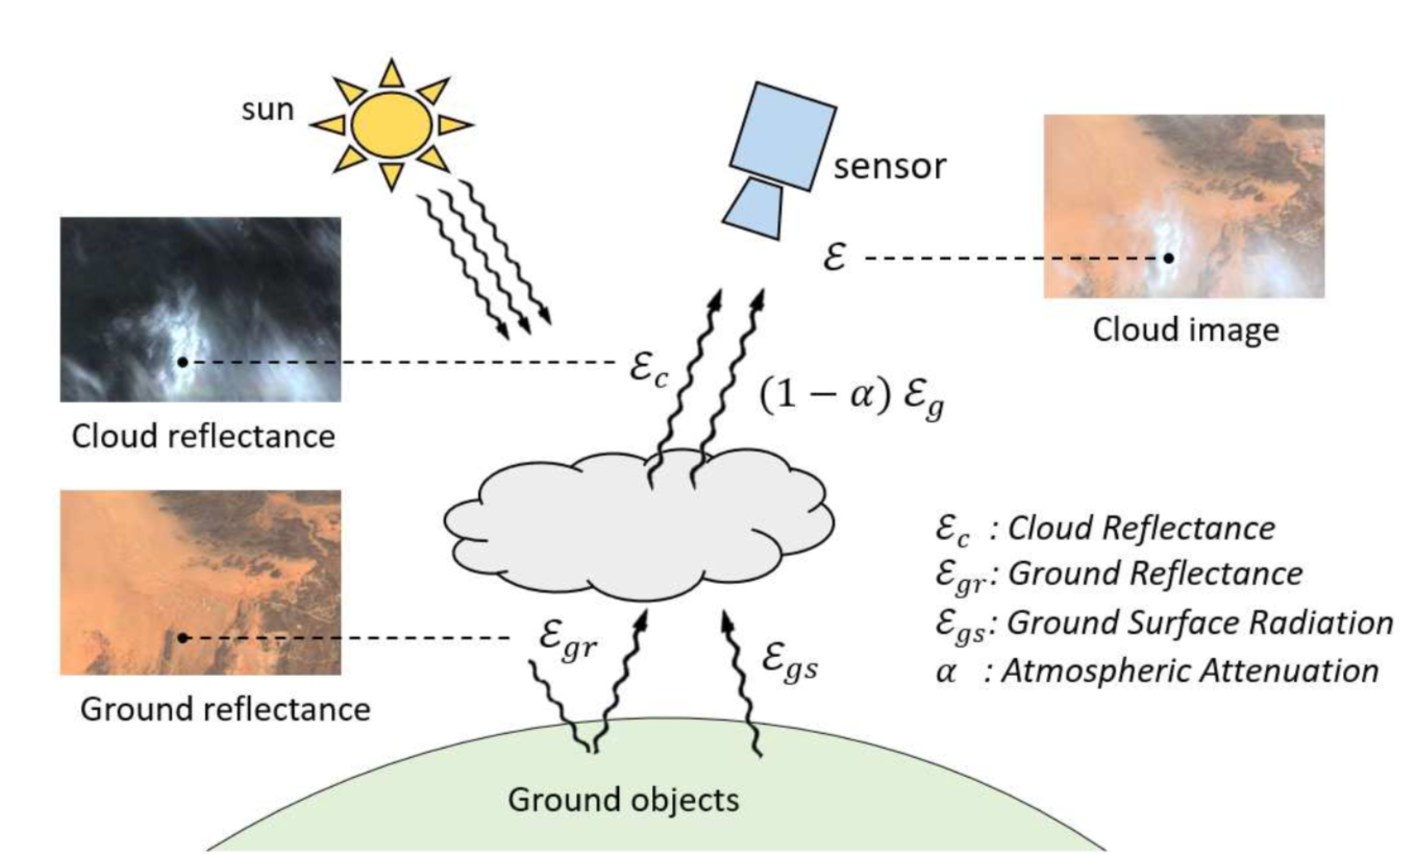
\includegraphics[width=0.75\textwidth]{images/cloud_matting_image}
\caption{Imaging model of cloud images.}
\end{figure}

\bibliographystyle{plain}
\bibliography{mybib}













\end{document}
